\section{Gravitational-Wave Signals from Binary Neutron Star Mergers}
\textcolor{blue}{Explain the use for this section.}\\
Gravitational waves from two inspiraling neutron stars are among the most interesting signals gravitational wave detectors can detect. They convey information about the highly relativistic regimes of gravity, about the structure of the component stars and about the formation channels of black holes or heavy neutron stars. \textcolor{red}{[Citations]} They are however also very hard to detect, as binary neutron star (\gls{bns}) systems are very light systems, when compared to inspiraling binary black holes (\gls{bbh}).\\
Part 1 of this section will discuss how gravitational waves (\gls{gw}) are formed and what influences the structure of the resulting waveforms. Part 2 will go over the current method of detecting \gls{gw} and discuss the advantages and drawbacks. \textcolor{red}{Need to specify, that I use Einstein sum convention in this section and that latin indices are spacial indices, whereas greek indices are over all four components. NEED TO CHANGE MOST CITATIONS FROM BACHELOR THESIS TO ORIGINAL SOURCES! Mention bachelor thesis only as a way to look up detailed calculations. Need to specify which convention is used for $\eta^\mn$. Look for ''energy-momentum-tensor'' and replace by ''energy-momentum tensor''. Search for ''chirp-mass'' and replace by ''chirp mass''. Through entire work replace ''decent'' with ''descent'' if some value goes down. (The other just means it was okay)}
\subsection{The Waveform}
\textcolor{blue}{Explain how the waveform looks like, what it depends on, maybe give the concept how it works in the context of linearized theory (quote bachelor thesis), cite important papers regarding the waveform theory.}\\
\subsubsection{Linearized Gravity}\label{sec:linearized_gravity}
Gravitational waves are a solution to the Einstein-equation
\begin{equation}\label{def:einstein_equation}
\mathcal{G}_\mn = \frac{8\pi G}{c^4}T_\mn,
\end{equation}
where $\mathcal{G}_\mn$ is the Einstein-tensor, $T_\mn$ is the energy-momentum-tensor, $G$ is the gravitational constant and $c$ is the speed of light in vacuum. They can be derived in their linear form by assuming the metric to be a linear correction to the flat metric $\eta_\mn$
\begin{equation}\label{def:linear_approximation}
g_\mn = \eta_\mn + h_\mn.
\end{equation}
With this approximation the Einstein-equation \eqref{def:einstein_equation} simplifies to
\begin{equation}\label{def:einstein_linear}
\mathcal{G}_\mn=\frac{1}{2}\lr{\partial_{\alpha\mu}h^\alpha_\nu+\partial^\alpha_\nu h_{\mu\alpha} - \partial_\mn h- \Box h_\mn - \eta_\mn\Box h} = \frac{8\pi G}{c^4}T_\mn,
\end{equation}
where $h\coloneqq\eta^\mn h_\mn$ and $\Box\coloneqq\eta^\mn\partial_\mn$.\\
This equation has $10$ independent components of which only $2$ are physical. To reduce the number of independent components, one can choose gauge conditions through the coordinate transformation ${x'}^\mu=x^\mu+\xi^\mu$, which leaves the Einstein equation invariant. One of these gauge conditions is the DeDonder gauge
\begin{equation}
\partial^\alpha \bar{h}_{\alpha\mu} = 0,
\end{equation}
where $\bar{h}_\mn\coloneqq h_\mn - \frac{1}{2}\eta_\mn h$. It can be realized by choosing $\Box\xi_\mu =\partial^\alpha \bar{h}_{\alpha\mu}$. In this gauge the linearized Einstein equation \eqref{def:einstein_linear} reduces to
\begin{equation}\label{def:gw_equation}
\Box\bar{h}_\mn=-\frac{16\pi G}{c^4}T_\mn.
\end{equation}
This gauge however doesn't fix $h_\mn$ completely, as another transformation ${x'}^\mu=x^\mu+\xi^\mu$ could be applied when $\Box\xi_\mu =0$. This can be used in a way that $\bar{h}=-h=0$ and $\bar{h}_{0\mu} = 0 = \bar{h}_{3\mu}$ are also satisfied. The gauge is named transverse-traceless-gauge (\gls{tt}) and results in the metric to be of the form
\begin{equation}\label{def:tt_gauge}
h_\mn^\text{\gls{tt}}=
\begin{pmatrix}
	0 & 0         & 0        & 0\\
	0 & h_+       & h_\times & 0\\
	0 & h_\times & -h_+      & 0\\
	0 & 0         & 0        & 0\\
\end{pmatrix}.
\end{equation}
\eqref{def:tt_gauge} now has only the two independent components $h_+$ and $h_\times$ left, which are called the ''plus-'' and ''cross-polarization'' of a \gls{gw}.\medskip\\
Evaluating \eqref{def:gw_equation} in vacuum reveals the wave-like character of $h_\mn$, as
\begin{equation}\label{def:gw_wave_equation}
\Box\bar{h}_\mn =0
\end{equation}
is a wave equation. Its solutions travel at the speed of light. Therefore, gravitational waves travel through space-time at the speed of light. The effect that a solution of this equation has on a ring of resting test masses is shown in \autoref{fig:gw_test_masses}. (chapter 3 \cite{bachelor})\medskip\\
\begin{figure}
\centering
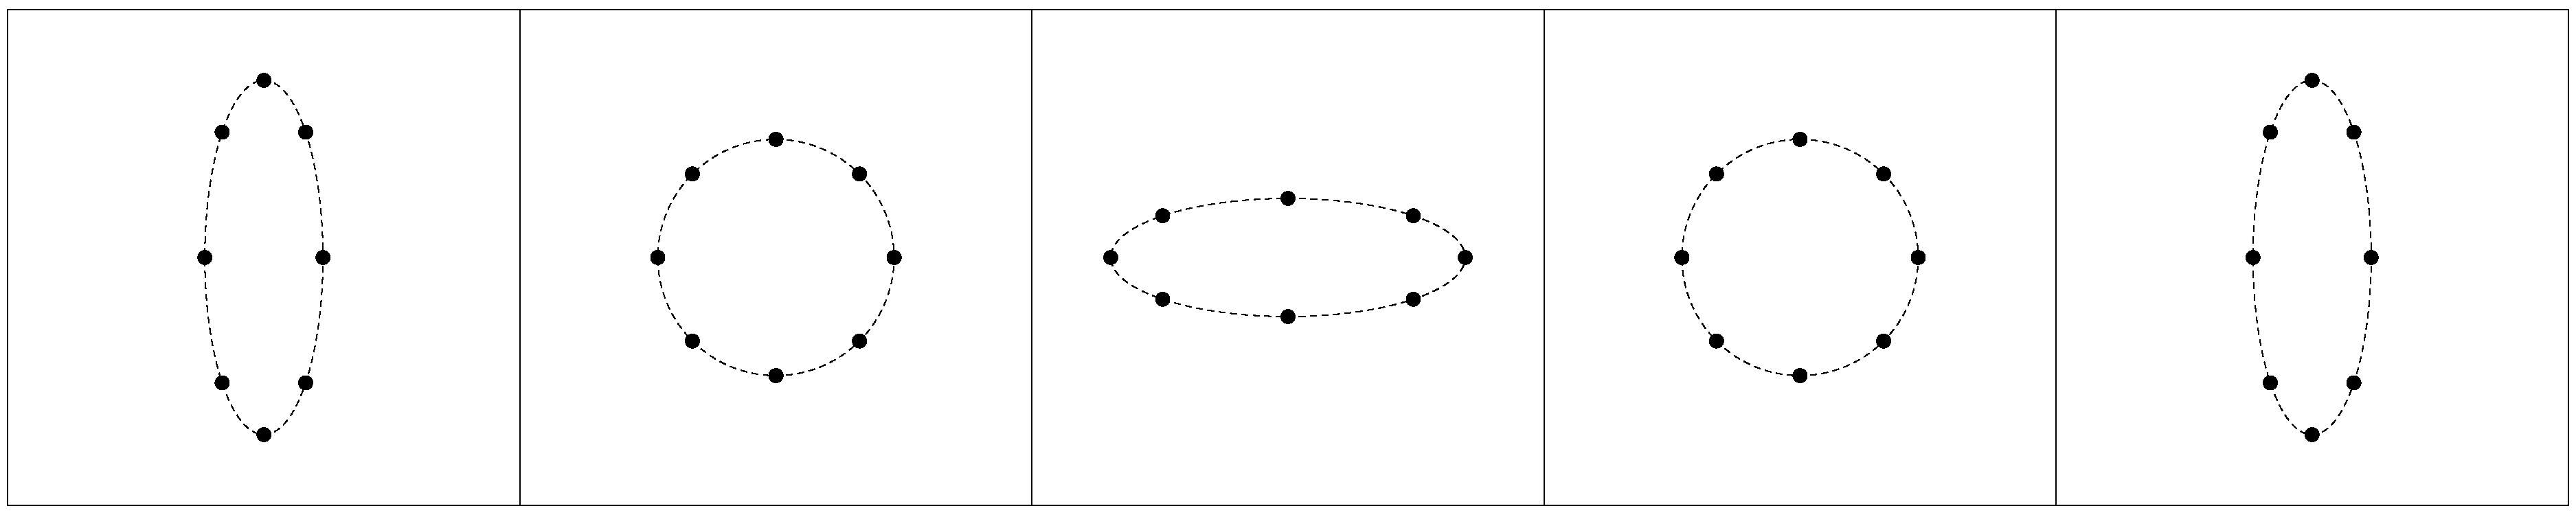
\includegraphics[width=\textwidth]{effect_gw.pdf}
\caption[Effect of GW on ring of test masses]{This image is taken from \cite{bachelor}. It shows the effect of a \gls{gw} passing orthogonally through a ring of test masses.}\label{fig:gw_test_masses}
\end{figure}
\eqref{def:gw_wave_equation} shows that \gls{gw} exist and can travel through space. It does, however, not specify how these waves are produced. To do so the energy-momentum-tensor cannot be set to $0$. Instead the full equation \eqref{def:gw_equation} needs to be solved. The solution is known to be
\begin{equation}
\bar{h}\lr{t, \vec{x}}=\frac{4 G}{c^4}\int\Diff{3}x'\ \frac{T_\mn\lr{t-\frac{\norm{\vec{x}-\vec{x}'}}{c},\vec{x}'}}{\norm{\vec{x}-\vec{x}'}}.
\end{equation}
For simplification, it is assumed that the observer is far away from the source when compared to the size of the support of $T_\mn$, such that $\norm{\vec{x}-\vec{x}'}\approx r\coloneqq\norm{\vec{x}}$. Therefore we need to solve
\begin{equation}
\bar{h}\lr{t, \vec{x}}=\frac{4 G}{c^4}\frac{1}{r}\int\Diff{3}x'\ T_\mn\lr{t-\frac{r}{c},\vec{x}'}.
\end{equation}
This equation can be solved to yield
\begin{equation}
h_{ab}^\text{\gls{tt}}\lr{t,\vec{x}}=\frac{2 G}{c^4}\frac{1}{r}\ddot{I}_{ab}^\text{\gls{tt}}\lr{t-r/c},
\end{equation}
where $\ddot{I}_{ab}^\text{\gls{tt}}$ is the transverse-traceless-projection of the second time derivative of the second mass moment
\begin{equation}\label{def:quad_st_1}
\ddot{I}^{ab}=c^2\partial_0^2 \int\Diff{3}x'\ x'^a x'^b T^{00} = 2\int\Diff{3}x'\ T^{ab}.
\end{equation}
As the quadrupole moment $Q_{ab}$ is simply the traceless second mass moment and we project it to its traceless part anyways, \eqref{def:quad_st_1} can be rewritten as
\begin{equation}\label{def:h_quadrupole}
\boxed{h^{\gls{tt}}_{ab}\lr{t,\vec{x}} = \frac{2 G}{c^4}\frac{1}{r}\ddot{Q}^{\gls{tt}}_{ab}\lr{t-r/c},}
\end{equation}
with $Q_{ab}\coloneqq I_{ab} - \frac{1}{3}\delta_{ab}I^c_c$. This is the famous quadrupole formula. (chapter 5.2 in \cite{bachelor})\medskip\\

\noindent To calculate the \gls{gw} a binary system emits, $I_{ab}$ or $Q_{ab}$ needs to be specified. Furthermore, the transverse-traceless-projection needs to be calculated. The projection turns out to be ((3.64) in \cite{gwv1})
\begin{equation}
\ddot{I}_{ab}^\text{\gls{tt}}=
\begin{pmatrix}
\lr{\ddot{I}_{11}-\ddot{I}_{22}}/2 & \ddot{I}_{12}                     & 0\\
\ddot{I}_{21}                      & -\lr{\ddot{I}_{11}-\ddot{I}_{22}}/2 & 0\\
0                                  & 0                                 & 0
\end{pmatrix}_{ab}.
\end{equation}
Therefore, the waveforms are given by
\begin{align}
h_+ & = \frac{1}{r}\frac{G}{c^4}\lr{\ddot{I}_{11}-\ddot{I}_{22}}\\
h_\times & = \frac{2}{r}\frac{G}{c^4}\ddot{I}_{12}.
\end{align}
The approximations that led to \eqref{def:einstein_linear} restrict the validity of the results above to cases where there are only slight perturbations to flat space-time. \eqref{def:linear_approximation} actually assumes the background to be flat. Therefore, the dynamics of the two bodies orbiting each other are dictated by Newtonian gravity. With this in mind, the binary system we are trying to model is a system of two point-particles with masses $m_1$, $m_2$. For simplicity\footnote{It turns out that this simplification is very accurate. This is due to two reasone. First of all a possibile ellipticity is radiated away before the \gls{gw} reaches currently detectable frequencies (4.1.3 in \cite{gwv1}). Secondly the rate of change of the orbital radius is small in the regime, where the approximation of linear gravity is meaningful. (4.1.1 in \cite{gwv1})} assume circular motion. In Newtonian mechanics, this problem reduces to an effective one body problem with the reduced mass $\mu=\frac{m_1m_2}{m_1+m_2}$. The motion in these relative coordinates is given by
\begin{equation}\label{def:binary_motion}
\vec{r}\lr{t} = R\cdot
\begin{pmatrix}
	-\sin\lr{\omega_s t}\\
	\cos\lr{\omega_s t}\\
	0
\end{pmatrix},
\end{equation}
where $R$ is the orbital separation of the two point masses and $\omega_s$ the orbital frequency. As a result one gets
\begin{equation}\label{def:binary_system_second_mass_moment}
\left[ I^{ab}\right] = \mu R^2\begin{pmatrix}
		\sin^2\lr{\omega_s t} & -\frac{1}{2}\sin\lr{2\omega_s t} & 0\\
		-\frac{1}{2}\sin\lr{2\omega_s t} & \cos^2\lr{\omega_s t} & 0\\
		0 & 0 & 0
	\end{pmatrix}
\end{equation}
and subsequently
\begin{equation}\label{def:binary_system_second_mass_moment_time_derivative}
\left[ \ddot{I}^{ab}\right] = 2 \mu R^2\omega_s^2
	\begin{pmatrix}
		\cos\lr{2\omega_s t} & \sin\lr{2\omega_s t} & 0\\
		\sin\lr{2\omega_s t} & -\cos\lr{2\omega_s t} & 0\\
		0 & 0 & 0
	\end{pmatrix}.
\end{equation}
Therefore, the amplitudes are given by
\begin{align}\label{def:gw_source_frame}
h_+ &= \frac{4}{r}\frac{G}{c^4}\mu R^2 \omega_s^2\cos\lr{2\omega_s t}\nonumber\\
h_\times &= \frac{4}{r}\frac{G}{c^4}\mu R^2 \omega_s^2\sin\lr{2\omega_s t}.
\end{align}
Interestingly, the frequency of the \gls{gw} is twice the frequency of the orbital period.\\
The equations \eqref{def:gw_source_frame} are written in the source frame, i.e. they are the \gls{gw}-polarizations emitted in the z-direction, where the z-axis is the one orthogonal to the orbital plane and at the center of mass. When measuring these waves we are not assured that the system emits face-on to our detectors. Therefore, we need to change coordinates to get the emission in a general direction $\hat{n}$. To do so, one simply has to transform the second mass moment into the new frame. These calculations can be found on p.111 in \cite{gwv1} which finally yield
\begin{align}\label{def:gw_travel_direction}
h_+ &= \frac{4}{r}\frac{G}{c^4}\mu R^2 \omega_s^2\lr{\frac{1+\cos^2\lr{\iota}}{2}}\cos\lr{2\omega_s t+2\Phi}\nonumber\\
h_\times &= \frac{4}{r}\frac{G}{c^4}\mu R^2 \omega_s^2\cos\lr{\iota}\sin\lr{2\omega_s t+2\Phi},
\end{align}
where $\iota$ is the inclination and $\Phi$ is the phase of the wave at $t=0$.\medskip\\
To be measured these waves need to hit a detector. The most common and currently only operational \gls{gw}-detectors are advanced Michelson interferometers with an angle of $\pi/2$ between the two arms. If the \gls{gw} hits such a detector, it will cause a deviation $\delta l$ in arm lengths given by the detector response functions
%\delta l = F_+\lr{\theta, \varphi} h_+ + F_\times\lr{\theta, \varphi} h_\times,
\begin{equation}\label{def:detector_response}
\delta l = F_+\lr{\theta, \varphi}\lr{\cos\lr{2\psi}h_+ - \sin\lr{2\psi} h_\times} + F_\times\lr{\theta, \varphi}\lr{\sin\lr{2\psi}h_+ + \cos\lr{2\psi} h_\times},
\end{equation}
with $h_+$ and $h_\times$ as given in \eqref{def:gw_travel_direction} and
\begin{align}
F_+\lr{\theta, \varphi} &\coloneqq \frac{1}{2}\lr{1+\cos^2\lr{\theta}}\cos\lr{2\varphi}\nonumber\\
F_\times\lr{\theta, \varphi} &\coloneqq\cos\lr{\theta}\sin\lr{2\varphi}.
\end{align}
The angle $\theta$ is the angle between the propagation direction of the \gls{gw} to the (outwards facing) normal of the detector. $\varphi$ is the angle between one arm of the detector\footnote{If the arms were labeled with $x$ and $y$ in such a way that they form a right handed coordinate system with the outwards facing normal vector, the arm the angle $\varphi$ is taken to is the one labeled $x$.} to the projection of the propagation direction of the \gls{gw} into the detector-plane. Therefore, the angles $\theta$ and $\varphi$, or rather their projection onto a global coordinate system, are the declination and right ascension respectively. The angle $\psi$ is known as the polarization angle and is not detectable for a single detector. This is due to the reason that rotating the wave around its propagation axis has the same effect.\medskip\\
All the calculations above disregarded the energy carried away by the \gls{gw}. To include it one needs to calculate the luminosity of a \gls{gw}-source, which in turn requires the computation of an effective energy-momentum tensor of the \gls{gw} itself.\\
To get this energy-momentum tensor, second order corrections in $h$ of $R_\mn$ need to be computed and averaged over time. The result is \textcolor{red}{[Citation]}
\begin{equation}
t_\mn = \frac{c^4}{32\pi G}\langle\partial_\mu h^{\sigma\alpha}\partial_\nu h_{\sigma\alpha}\rangle.
\end{equation}
The luminosity is the energy flux at spatial infinity and thus given by
\begin{equation}
L_\text{\gls{gw}} = \lim_{r\to\infty}\int_{S^2\lr{r}}\diff\vec{n}\ \vec{S},
\end{equation}
where $S^i=-c\cdot t^{0i}$ and $S^2\lr{r}$ denotes the spherical shell of radius $r$. When solving this integral and using \eqref{def:h_quadrupole} one gets
\begin{equation}\label{def:luminosity_quadrupole}
\boxed{L_\text{\gls{gw}}=\frac{G}{5c^5}\langle\dddot{Q}^{ab}\dddot{Q}_{ab}\rangle.}
\end{equation}
This equation can now be applied to the binary system specified by \eqref{def:binary_system_second_mass_moment}. To simplify notation and to give measurable parameters, notice that the dynamics of the system under consideration are governed by Newtonian physics and thus Kepler's laws apply. Especially Kepler's third law
\begin{equation}\label{def:kepler_third_law}
\omega_s^2=\frac{G M}{R^3}
\end{equation}
will be of use, where $M=m_1+m_2$ is the total mass of the system. Using \eqref{def:kepler_third_law} to eliminate $R$ in \eqref{def:binary_system_second_mass_moment} and inserting this equation into \eqref{def:luminosity_quadrupole} yields
\begin{equation}\label{def:luminoisity_binary_system}
L_\text{\gls{gw}}=\frac{32}{5}\frac{c^5}{G}\lr{\frac{G\omega_s M_c}{c^3}}^{10/3},
\end{equation}
where
\begin{equation}
M_c\coloneqq \mu^{3/5}M^{2/5}=\frac{\lr{m_1 m_2}^{3/5}}{\lr{m_1 + m_2}^{1/5}}.
\end{equation}
$M_c$ is called the chirp mass and is the only mass-combination a \gls{gw} depends on in linearized theory.\medskip\\
According to \eqref{def:luminoisity_binary_system}, a binary system looses energy when emitting \gls{gw}. The energy that is carried away is taken from the orbital energy $E_\text{orbit}$ of the binary system. Therefore, disregarding any other effects\footnote{These effects could for instance be tidal deformation, mass acquisition or other sources of gravity in the proximity of the binary system.} that might cause $E_\text{orbit}$ to vary, we get
\begin{equation}
-\frac{d E_\text{orbit}}{dt}=-\frac{1}{2}\frac{G m_1 m_2 \dot{R}}{R^2}\mbe L_\text{\gls{gw}}.
\end{equation}
One can again utilize \eqref{def:kepler_third_law} to eliminate $R$ and $\dot{R}$ in favor of $\omega_s$ and $\dot{\omega}_s$. Furthermore, $\omega_s = \pi f_\text{\gls{gw}}$, and thus
\begin{equation}\label{def:frequency_evolution_differential}
\dot{f}_\text{\gls{gw}}=\frac{96}{5}\pi^{8/3}\lr{\frac{G M_c}{c^3}}^{5/3}f_\text{\gls{gw}}^{11/3}.
\end{equation}
This equation describes a runaway process, as for a positive value $f_\text{\gls{gw}}$ the change in frequency is positive, leading to a larger value of $f_\text{\gls{gw}}$ and so on. This in turn by \eqref{def:kepler_third_law} means that the two masses will come closer and closer together until they touch. The point in time at which the waveform shuts off, will be denoted by $t_\text{coal}$. With this, one can define the time until coalescence $\tau=t_\text{coal}-t$ and solve the differential equation \eqref{def:frequency_evolution_differential}. \textcolor{red}{[Cite p.170 \cite{gwv1}]}
\begin{equation}\label{def:frequency evolution}
f_\text{\gls{gw}}\lr{\tau} = \frac{1}{\pi}\lr{\frac{5}{256}\frac{1}{\tau}}^{3/8}\lr{\frac{G M_c}{c^3}}^{-5/8}
\end{equation}
Now that the frequency evolution of a \gls{gw} is known, the amplitudes $h_+$ and $h_\times$ can also be modeled. To do so, revisit the initial assumption \eqref{def:binary_motion}. In this equation $R$ will now be time dependent and $\omega_s t$ will be replaced by $\Phi\lr{t}$, where
\begin{equation}\label{def:phase_equation}
\Phi\lr{t} = 2\pi \int_{t_0}^t\diff t'\ f_\text{\gls{gw}}\lr{t'}.
\end{equation}
In principle, all time derivatives in \eqref{def:binary_system_second_mass_moment_time_derivative} would need to be redone, taking into account the time dependence of $\omega_s$ and $R$. However, the approximations that have led to these waveforms are quite strong. The rates of change $\dot{\omega}_s$ and $\dot{R}$ will only have non-negligible contributions when frequencies are pretty high and the orbital separation $R$ is small. In these regimes the linear approximation \eqref{def:linear_approximation} will be invalid. Therefore, we can neglect the contributions of $\dot{\omega}_s$ and $\dot{R}$ and still get a qualitative look into the dynamics of the system. Hence, replace $\omega_s$ in the prefactor of \eqref{def:gw_travel_direction} by $\pi f_\text{\gls{gw}}\lr{t}$, $2\omega_s t + 2 \Phi$ by $\Phi\lr{t}$ and $R$ by \eqref{def:kepler_third_law}.\\
With \eqref{def:frequency evolution}, equation \eqref{def:phase_equation} can be solved to yield
\begin{equation}
\Phi\lr{\tau}=-2\lr{\frac{5 G M_c}{c^3}}^{-5/8}\tau^{5/8}+\Phi_0,
\end{equation}
where $\Phi_0$ is the phase at $\tau=0$, i.e. at coalescence. Therefore, this value is called the coalescence phase. Combining these results, one gets the time dependent waveforms
\begin{align}\label{def:linear_waveforms_time_evolution}
h_+\lr{t} & = \frac{1}{r}\lr{\frac{G M_c}{c^2}}^{5/4}\lr{\frac{5}{c\tau}}^{1/4}\lr{\frac{1+\cos^2\lr{\iota}}{2}}\cos\lr{\Phi\lr{\tau}}\nonumber\\
h_\times\lr{t} & = \frac{1}{r}\lr{\frac{G M_c}{c^2}}^{5/4}\lr{\frac{5}{c\tau}}^{1/4}\cos\lr{\iota}\cos\lr{\Phi\lr{\tau}}.
\end{align}
Inserting \eqref{def:linear_waveforms_time_evolution} and \eqref{def:detector_response} shows that in linearized theory the output of a detector depends on 8 parameters. These are the luminosity distance $r$, the chirp mass $M_c$, the coalescence time $t_\text{coal}$, the coalescence phase $\Phi_0$, the inclination $\iota$, the declination $\theta$, the right ascension $\varphi$ and the polarization angle $\psi$. The first four parameters are source intrinsic parameters, where $M_c$ is a combination of the component masses $m_1$ and $m_2$. In that sense the parameter space can be extended to be 9-dimensional.\\
\autoref{fig:linear_waveform} shows an example of the time evolution of a waveform described by \eqref{def:linear_waveforms_time_evolution}. \textcolor{red}{To obtain the spin effects in linearized gravity, one could write down the lagrangian of two spinning particles orbiting each other, solving the lagrange equation for the trajectories of the particles and insert these trajectories into the definition of the quadrupole tensor. (At least that's how I think it could be done. If there is time, maybe do these calculations.)}\\
Alongside energy, \gls{gw} also carry away angular momentum from the source. Using the quadrupole radiation \eqref{def:h_quadrupole}, the change in angular momentum evaluates to ((3.97) in \cite{gwv1})
\begin{equation}
\frac{dJ^i}{dt}=\frac{2G}{c^5}\varepsilon^{ikl}\langle \ddot{Q}_{ka}\dddot{Q}_{la}\rangle .
\end{equation}
The angular momentum that is carried away comes from the total angular momentum of the source. This in turn is comprised of the orbital angular momentum as well as the individual spins of the two component masses of a binary system. Therefore it is at least qualitatively understandable that the spins of the two bodies has an effect on the evolution of the waveform. Thus the 9 parameters of a waveform can be extended to 15, if both objects are allowed to rotate. The 6 additional parameters are the individual angular momenta of the two masses. Two further parameters influence the waveform if the objects are not rigid and allowed to deform. This is true for binary neutron stars, as neutron stars are not singularities.\\
Even though this work deals with \gls{bns}-signals, we neglect spin effects and tidal deformability and will thus not go into further detail here. \textcolor{red}{For more information on spin- and tidal effects see [Citations].}\\
\begin{figure}
\centering
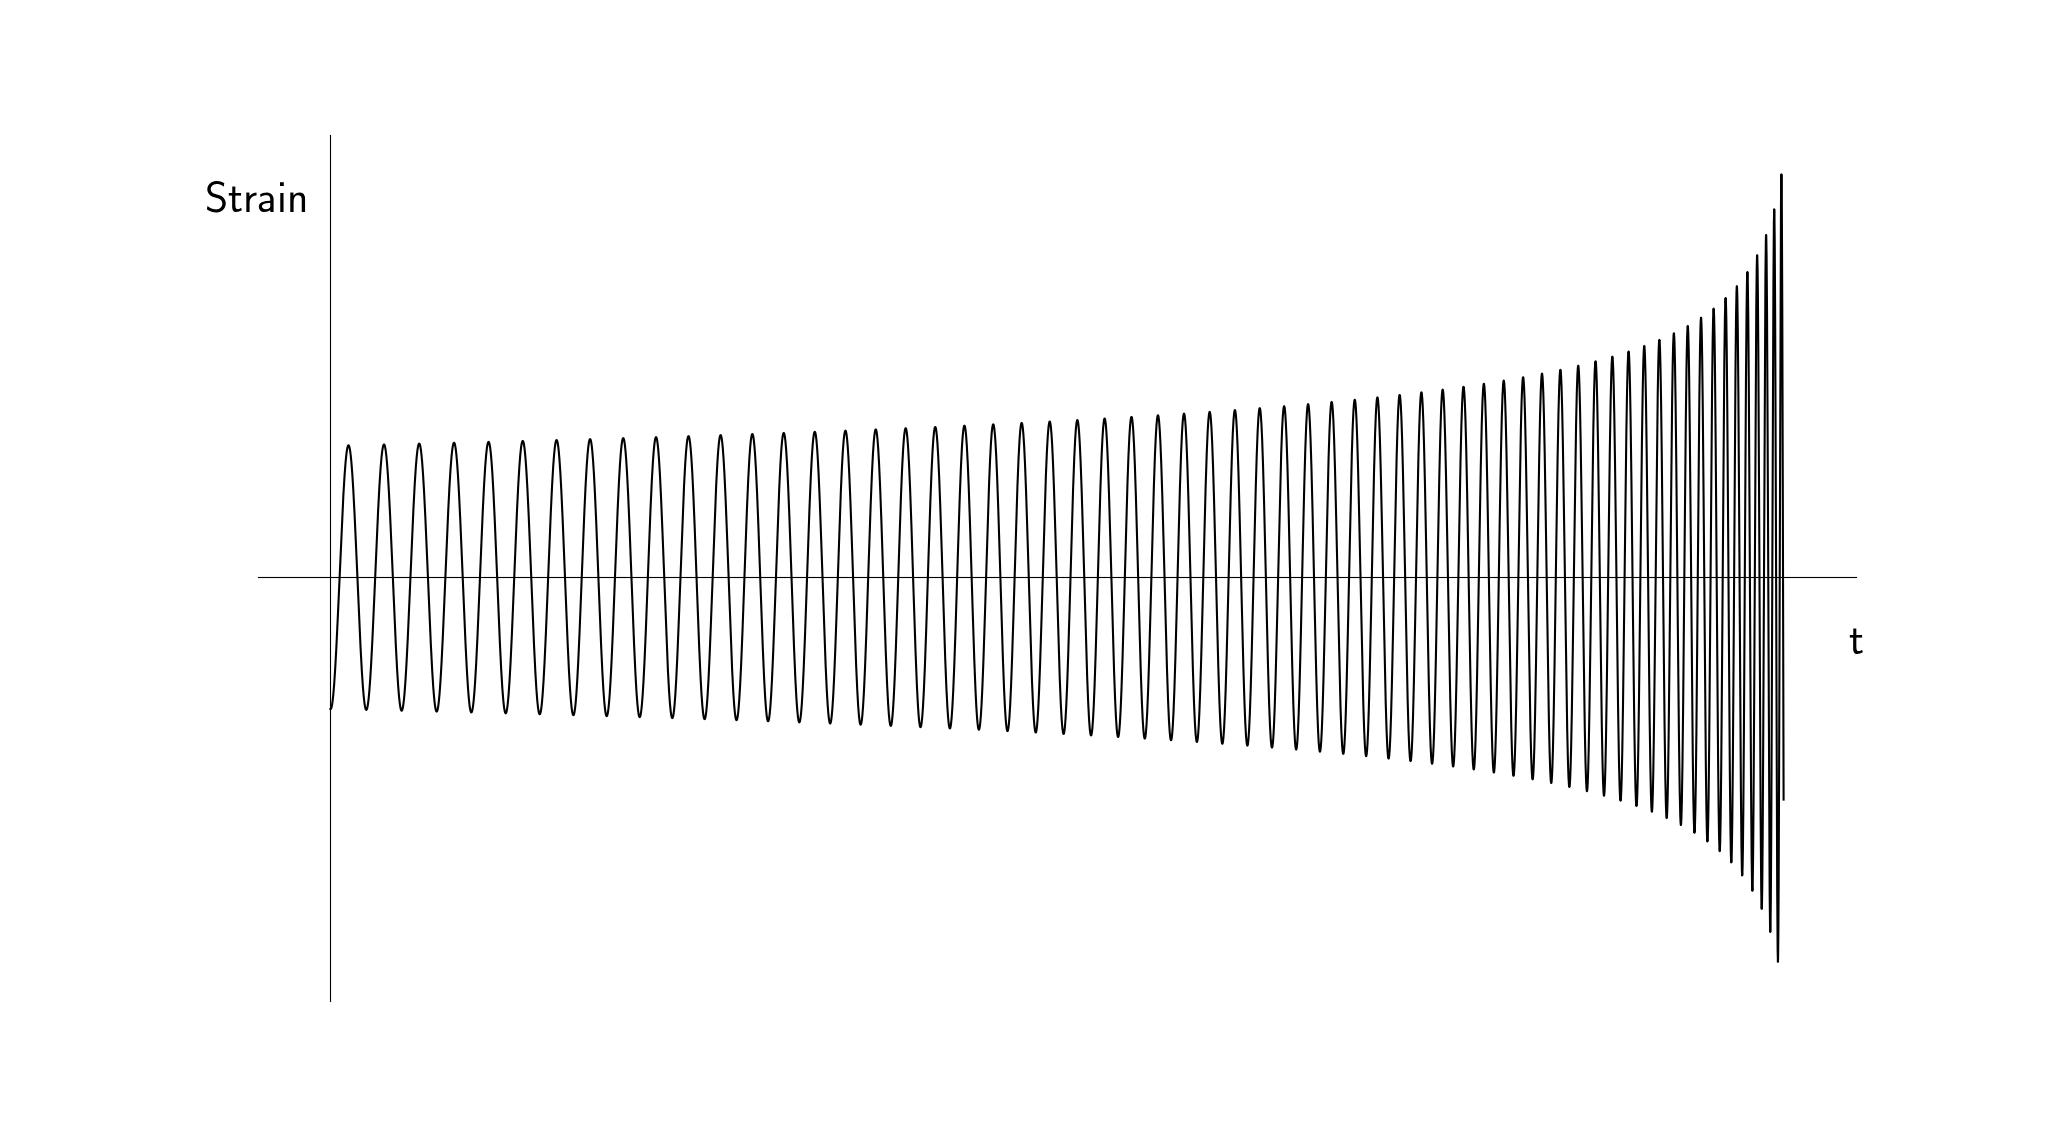
\includegraphics[width=\textwidth]{linear_waveform.png}
\caption[Example time-evolution of a linear waveform]{This figure is heavily based on Figure 4.1 in \cite{gwv1}. Shown is an example of a waveform as it could be observed by a detector if the linear waveforms describe the source accuratly. Note the frequency and amplitude evolution, they both rise simultaniously. This behavior is called ''chirping''.}\label{fig:linear_waveform}
\end{figure}

\subsubsection{Post-Newtonian Expansion}\label{sec:pn_expansion}
This part closely follows chapter 5 in \cite{gwv1}, mainly stating results and concepts.\\
As we will see in \autoref{sec:matched_filtering}, accurate models for the waveforms are necessary to detect \gls{gw} using traditional methods. This condition is not dropped for an approach utilizing machine learning algorithms, as they can only detect waveforms from distributions they have sampled before. \textcolor{red}{Citation?} Though the waveform derived in \eqref{def:linear_waveforms_time_evolution} gives a good qualitative overview of the rough amplitude evolution of inspiraling binary systems, it is hardly an accurate model. The main drawback of this model are the dynamics used to describe the motion of the system. It assumed \eqref{def:linear_approximation} which in turn means that \gls{gws} and source-dynamics can be separated. Therefore, in linearized gravity the motion of a binary system is dictated by Newtonian dynamics, while the \gls{gws} are a relativistic effect.\\
This issue is overcome, by taking an approach called post-Newtonian expansion (\gls{pn}-expansion). To approximate the solution of the full Einstein equation \eqref{def:einstein_equation}, $g_\mn$ is expanded in powers of the small parameter $\epsilon\sim v/c \sim \lr{R_s / d}^{1/2}$, instead of using $g_\mn\approx h_\mn +\eta_\mn$. Here $v$ is the typical speed inside the source, $R_s$ is the Schwarzschild radius attributed to the system's total mass and $d$ is the diameter of a world-tube containing the support of the energy-momentum-tensor of the source. Therefore, $\epsilon$ is small if the source is not too compact and speeds are low compared to the speed of light.\\
Specifically the metric expands to \textcolor{red}{(Mention why they start at different orders?)}
\begin{align}\label{def:pn_expansion_metric}
g_{00} && = & -1 && +{g^{(2)}}_{00} & +{g^{(4)}}_{00} && +{g^{(6)}}_{00} && +\dotsc\nonumber\\
g_{0j} && = & && & +{g^{(3)}}_{0j} && +{g^{(5)}}_{0j} && +\dotsc\\
g_{ij} && = & &&\delta_{ij} & +{g^{(2)}}_{ij} && +{g^{(4)}}_{ij} && +\dotsc,\nonumber
\end{align}
where ${g^{(n)}}$ denotes a term $\sim \epsilon^n$. The energy-momentum-tensor can be expanded in an equivalent way
\begin{align}\label{def:pn_expansion_energy_momentum_tensor}
T^{00} & = {T^{(0)}}^{00}+{T^{(2)}}^{00}+\cdots\nonumber\\
T^{0i} & = {T^{(1)}}^{0i}+{T^{(3)}}^{0i}+\cdots\\
T^{ij} & = {T^{(4)}}^{ij}+{T^{(4)}}^{ij}+\cdots.\nonumber
\end{align}
These expressions than need to be inserted into \eqref{def:einstein_equation} and terms of the same order in $\epsilon$ need to be equated. To get the equations of motion to the $n$-th \gls{pn}-order terms up to order $\epsilon^{2n}$ need to be kept and computed. Therefore it is possible to have the correction of some quantity to \gls{pn}-order $2.5$.\\
To get the 1-\gls{pn} order corrections to the metric, one can once again impose a gauge condition. \textcolor{red}{Gauge condition can be required for any order.} The gauge condition most commonly used is still called deDonder gauge, which in the \gls{pn}-case reads
\begin{equation}
\partial_\mu\lr{\sqrt{-g}g^\mn}=0,
\end{equation}
where $g$ is the determinant of $g_\mn$. In this gauge the Einstein equation yields (to 1-\gls{pn} order)
\begin{align}\label{def:metric_differential_equation_pn_1}
\Delta {g^{(2)}}_{00} = & -\frac{8\pi G}{c^4}{T^{(0)}}^{00}\nonumber\\
\Delta {g^{(2)}}_{ij} = & -\frac{8\pi G}{c^4}\delta_{ij}{T^{(0)}}^{00}\nonumber\\
\Delta {g^{(3)}}_{0i} = & \frac{16\pi G}{c^4}{T^{(1)}}^{0i}\\
\Delta {g^{(4)}}_{00} = & \partial_0^2{g^{(2)}}_{00} + {g^{(2)}}_{ij}\partial_i\partial_j{g^{(2)}}_{00}-\partial_i{g^{(i)}}_{00}\partial_j{g^{(2)}}_{00}\nonumber\\
& -\frac{8\pi G}{c^4}\left\{{T^{(2)}}^{00}+{T^{(2)}}^{ii}-2{g^{(2)}}_{00}{T^{(0)}}{00}\right\},\nonumber
\end{align}
with $\Delta = \delta^{ij}\partial_i\partial_j$. Observe that higher order terms in \eqref{def:metric_differential_equation_pn_1} depend on the lower order terms of the expansion. Therefore the \gls{pn}-expansion is an iterative process.\\
The equations \eqref{def:metric_differential_equation_pn_1} do in principle have a solution. The specific solution however depends on the boundary condition. A typical boundary condition is the ''no incoming radiation'' condition, where it is required that the metric vanishes at spatial infinity. The \gls{pn}-expansion however is only valid in the near region of the source, as it approximates the retarded solutions by a series of instantaneous potentials. To use a correct boundary condition one approximates the far-field solution and matches it with the near-field \gls{pn}-solution.\\
The approximation for the far-field is called Post-Minkowskian-expansion (\gls{pm}-expansion). For simplified notation the Einstein equation will be recast into their relaxed form
\begin{equation}\label{def:einstein_equation_relaxed}
\Box k^\mn = \frac{16\pi G}{c^4}\tau^\mn.
\end{equation}
To get this result, the deDonder gauge
\begin{equation}
\partial_\nu k^{\mn}=0
\end{equation}
was again required. The metric $k$ is given by
\begin{equation}
k^\mn\coloneqq \sqrt{-g}g^\mn -\eta^\mn.
\end{equation}
Furthermore
\begin{equation}\label{def:pn_tau}
\tau^\mn = \lr{-g}T^\mn + \frac{c^4}{16\pi G}\Lambda^\mn,
\end{equation}
with $\Lambda^\mn$ being a tensor that depends highly nonlinearly on $k$ and $g$. The expression is given in (5.74) of \cite{gwv1}. To simplify the relaxed Einstein equation \eqref{def:einstein_equation_relaxed} in the far field, we denote that the energy-momentum-tensor of matter $T^\mn$ vanishes outside the source. Therefore the task is solving
\begin{equation}
\Box k^\mn = \Lambda^\mn.
\end{equation}
To do so, we expand $k$ in powers of $R_s/r$, which is equivalent to expanding in powers of $G$. We also expand $\Lambda^\mn$ in powers of $k$. Therefore
\begin{gather}
k^\mn=\sum_{n=1}^\infty G^n k^\mn_n\\
\Lambda^\mn = N^\mn\left[k,k\right] + M^\mn\left[k,k,k\right]+\dotsc.
\end{gather}
Equating terms of the same order in $G$ and iteratively using the results for $k$ yields
\begin{gather}
\Box k^\mn_1=0\\
\Box k^\mn_2 = N^\mn\left[k_1, k_1\right]\\
\Box k^\mn_3 = M^\mn\left[k_1, k_1, k_1\right]+N^\mn\left[k_1,k_2\right]+N^\mn\left[k_2,k_1\right]\\
\vdots\nonumber
\end{gather}
or in short
\begin{equation}\label{def:pm_wave_equation}
\Box k^\mn_n=\Lambda^\mn_n\left[k_1, \dotsc, k_{n-1}\right].
\end{equation}
The most general solution to $k_1$ can be written in terms of retarded multipolar waves. The solution under consideration of the deDonder gauge can be found in equation (5.95) and following of \cite{gwv1}. They consist of multiple retarded potentials and form a multipole expansion of $k_1$. To find the solution to any order $n$ equation \eqref{def:pm_wave_equation} needs to be solved, inserting all previous solution $k_1,\dotsc,k_{n-1}$. Therefore, a general solution to \eqref{def:pm_wave_equation} would be convenient.\\
Traditionally such a solution is known and given by the retarded Green's function. The problem, however, is that the solution to \eqref{def:pm_wave_equation} is only valid outside the source but solving it by the retarded Green's function requires knowledge over the entire region. To get around this issue, we observe the fact that we only want the solution of $k$ to some finite order in $G$. This has the benefit that only a finite number of multipole terms of $\Lambda^\mn_n$ have to be used. The finite number of terms enables us to find some constant $B$, such that $r^B\Lambda^\mn_n$ is defined for all $r$ and thus its solution is given by the retarded Green's function. For $B\to 0$ the original divergence is recovered and the multipole expansion has poles. Therefore, near $B=0$ the solution $I^\mn_n\lr{B}=\Box^{-1}_\text{ret}\lr{r^B\Lambda^\mn_n}$ can be expanded in a Laurent-series. Taking only the zeroth order term yields a particular solution $u^\mn_n$ with
\begin{equation}
\Box u^\mn_n=\Lambda^\mn_n.
\end{equation}
From this particular solution the general solution can be constructed by adding the homogeneous solution.\medskip\\
As a final step, the \gls{pn}-expansion can be recast in the form of $k$, where we expand
\begin{gather}
k_\mn =\sum_{n=2}^\infty \frac{1}{c^n}\frac{d^n}{du^n}k_\mn\lr{u}\\
\tau^\mn=\sum_{n=2}^\infty \frac{1}{c^n}\frac{d^n}{du^n}\tau^\mn\lr{u},
\end{gather}
with $u=t-r/c$ and $\tau$ given in \eqref{def:pn_tau}. Doing so and inserting it into the relaxed Einstein equations results in the recursive relation
\begin{equation}\label{def:k_solution_pn}
\Delta\left[\frac{d^n}{du^n}k^\mn\right]=16\pi G\frac{d^{n-4}}{du^{n-4}}\tau^\mn+\partial_t^2\left[\frac{d^{n-2}}{du^{n-2}}k^\mn\right].
\end{equation}
Taking the solution for the 1\gls{pn} case discussed above as a starting point the \eqref{def:k_solution_pn} can be solved in a similar fashion to \eqref{def:pm_wave_equation} using only a finite number of terms in a multipole expansion of the potentials.\medskip\\
With this setup we mention once more that the regions of validity for the \gls{pn}- and \gls{pm} expansion overlap but neither are completely solved. To obtain the full solution the \gls{pn}-equations need a boundary condition, whereas the \gls{pm}-equations need a source of some form. Therefore the \gls{pm}-equations can be viewed as the limiting case of the \gls{pn}-case and thus provide a boundary condition. The \gls{pn}-equations on the other hand have fixed multipole potentials that depend on the energy-momentum tensor of matter. These can in turn be used to fix the multipole potentials in the \gls{pm}-equations and one obtains a full solution.\\
At this point we will not go further into further details of the formalism itself but rather look at its influence on the waveforms. \textcolor{red}{For further reference on the PN-formalism see [Citations]. For information about the multipole expansion see [Citations].}\medskip\\
Surprisingly, to 1\gls{pn} order the results are identical to the ones obtained using linearized gravity in \autoref{sec:linearized_gravity}. For convenience one defines the dimensionless quantity
\begin{equation}
x\coloneqq \lr{\frac{G M \omega_s}{c^3}}^{2/3},
\end{equation}
where $M$ is the total mass and $\omega_s$ the orbital frequency. Note that $x\sim \frac{v^2}{c^2}$ and thus the \gls{pn}-expansion can be given in terms of powers in $x$. For further notational simplicity define the symmetric mass ratio
\begin{equation}
\nu\coloneqq \frac{m_1 m_2}{\lr{m_1 + m_2}^2},
\end{equation}
the post-Newtonian parameter
\begin{equation}
\gamma\coloneqq \frac{G M}{r c^2}
\end{equation}
and the dimensionless time parameter \textcolor{red}{Maybe remove $\theta$ as it is not used.}
\begin{equation}
\Theta\coloneqq \frac{\nu c^3}{5 G M}\lr{t_\text{coal}-t}.
\end{equation}
Using the metrics acquired from the \gls{pn}-expansion one can solve the equations of motion for the two inspiraling bodies and obtain corrections to $\omega_s$, $\gamma$, the energy $E$ and the radiated power $L_\text{\gls{gw}}$. Combining these results one can than find the phase evolution and emitted waveforms. The computations are extremely long. For this reason we only state the results for the energy and luminosity at $3.5$\gls{pn} order here. ($\mu$ in this case is the reduced mass) (equation (5.256) in \cite{gwv1})
\begin{align}
E= & -\frac{\mu c^2 x}{2}\left\{ 1+\lr{-\frac{3}{4}-\frac{1}{12}\nu}x+\lr{-\frac{27}{8}+\frac{19}{8}\nu-\frac{1}{24}\nu^2}x^2\right.\nonumber\\
& +\left. \left[ -\frac{675}{64}+\lr{\frac{34445}{576}-\frac{205}{96}\pi^2}\nu -\frac{155}{96}\nu^2 - \frac{35}{5184}\nu^3\right] x^3\right\}+\mathcal{O}\lr{\frac{1}{c^8}}
\end{align}
In the equation below $C$ is the Euler-Mascheroni constant. (equation (5.257) in \cite{gwv1})
\begin{align}
L_\text{\gls{gw}} = & \frac{32 c^5}{5 G}\nu^2 x^5 \left\{ 1 + \lr{-\frac{1247}{336}-\frac{35}{12}\nu}x + 4\pi x^{3/2}\right.\nonumber\\
& + \lr{-\frac{44711}{9072}+\frac{9271}{504}\nu+\frac{65}{18}\nu^2}x^2\nonumber\\
& + \lr{-\frac{8191}{672}-\frac{583}{24}\nu}\pi x^{5/2}\nonumber\\
& + \left[ \frac{6643739519}{69854400}+\frac{16}{3}\pi^2 -\frac{1712}{105}C-\frac{856}{105}\log\lr{16 x}\right.\nonumber\\
& + \left. \lr{-\frac{134543}{7776}+\frac{41}{48}\pi^2}\nu - \frac{94403}{3024}\nu^2 - \frac{775}{324}\nu^3\right] x^3\nonumber\\
& + \left. \lr{-\frac{16258}{504}+\frac{214745}{1728}\nu + \frac{193385}{3024}\nu^2}\pi x^{7/2}+\mathcal{O}\lr{\frac{1}{c^8}}\right\}
\end{align}

\subsubsection{TaylorF2}
Even though the \gls{pn}-formalism allows us to model the waveforms rather accurately for a long part of the signal it still assumes circular motion and velocities to be small. As the two stars spiral together they will, however, reach a point, where circular motion is not possible anymore. This orbit is called the ''innermost stable circular orbit'' (\gls{isco}). From here the stars will plunge towards each other, velocities are high and fields are not weak anymore. Therefore, the validity of the formalism breaks down at this point. Finally, after the two bodies have merged, the remaining body will radiate off some more energy. Therefore, the signal consists of three parts: inspiral, merger and ringdown. The inspiral phase is well modeled by the \gls{pn}-formalism outlined in \autoref{sec:pn_expansion}. The ringdown can be described by \textcolor{red}{What can it be described by and where can one find an analysis of this?} The merger however is very difficult to model and usually involves numerical solutions of the Einstein equations. These, however, are very costly from a computational perspective, which is a great problem when one searches for \gls{gws}.
\textcolor{red}{Transition into roughly describing the PN-approximation and TaylorF2 here.}
%Until now, the approximations made were quite strict. One of the major ones is the approximation of the two bodies of mass $m_1$ and $m_2$ as point particles. As such they have no intrinsic spin. Dropping this restriction shows, that also angular momentum is radiated away. Also each \textcolor{red}{Spin seems to be difficult. If it doesn't fit time wise, consider just pointing out, that there are in theory 6 more parameters coming from the individual spins, but as we only look at non-spinning systems anyways, we will not go into further detail and the effects here. Otherwise maybe look at Stephans Bachelor thesis to get a little grasp on spins and their effects? However I'm not comfortable writing, that spins only come into effect in PN-theory. Maybe I can find a mass momentum $I^{ab}$ for a binary system of two spinning masses and just say, that this can be plugged into the according equations?}\\
\textcolor{red}{Include backreaction in first order as 4.1.1 \cite{gwv1} does, until equation (4.32). Mention that elliptic effects can be mostly disregarded, cite \cite{gwv1}. Go over into PN territory and mention what changes.}

\subsection{Searching for Gravitational Waves}\label{sec:matched_filtering}
\textcolor{blue}{Explain what matched filtering is, why it works and how it is applied currently. Also need to mention PSD and what it is.}